%% ENGR114_lab_assignment.tplx %%
%
% Built off of the article.tplx template %


% Default to the notebook output style

    


% Inherit from the specified cell style.




    
    \documentclass[11pt]{article}

    
    
    %% installed packages_rev2.tplx %%

\usepackage{fancyhdr}
\usepackage{lastpage}
\usepackage{framed,color}
\definecolor{shadecolor}{rgb}{.8,.8,.8}
\usepackage{titlesec}
% no indent on any paragraphs, vertical spacing between paragraphs is set to 1em
\usepackage[]{parskip}  % add [skip=1em] if the compiler will allow.

% for MATLAB syntax highlighting
\usepackage{listings}             % Include the listings-package
\definecolor{mygray}{rgb}{0.8,0.8,0.8} % color values Red, Green, Blue
\definecolor{mygreen}{RGB}{28,172,0}
\definecolor{mylilas}{RGB}{170,55,241}
    
    \usepackage[T1]{fontenc}
    % Nicer default font (+ math font) than Computer Modern for most use cases
    \usepackage{mathpazo}

    % Basic figure setup, for now with no caption control since it's done
    % automatically by Pandoc (which extracts ![](path) syntax from Markdown).
    \usepackage{graphicx}
    % We will generate all images so they have a width \maxwidth. This means
    % that they will get their normal width if they fit onto the page, but
    % are scaled down if they would overflow the margins.
    \makeatletter
    \def\maxwidth{\ifdim\Gin@nat@width>\linewidth\linewidth
    \else\Gin@nat@width\fi}
    \makeatother
    \let\Oldincludegraphics\includegraphics
    % Set max figure width to be 80% of text width, for now hardcoded.
    \renewcommand{\includegraphics}[1]{\Oldincludegraphics[width=.8\maxwidth]{#1}}
    % Ensure that by default, figures have no caption (until we provide a
    % proper Figure object with a Caption API and a way to capture that
    % in the conversion process - todo).
    \usepackage{caption}
    \DeclareCaptionLabelFormat{nolabel}{}
    \captionsetup{labelformat=nolabel}

    \usepackage{adjustbox} % Used to constrain images to a maximum size 
    \usepackage{xcolor} % Allow colors to be defined
    \usepackage{enumerate} % Needed for markdown enumerations to work
    \usepackage{geometry} % Used to adjust the document margins
    \usepackage{amsmath} % Equations
    \usepackage{amssymb} % Equations
    \usepackage{textcomp} % defines textquotesingle
    % Hack from http://tex.stackexchange.com/a/47451/13684:
    \AtBeginDocument{%
        \def\PYZsq{\textquotesingle}% Upright quotes in Pygmentized code
    }
    \usepackage{upquote} % Upright quotes for verbatim code
    \usepackage{eurosym} % defines \euro
    \usepackage[mathletters]{ucs} % Extended unicode (utf-8) support
    \usepackage[utf8x]{inputenc} % Allow utf-8 characters in the tex document
    \usepackage{fancyvrb} % verbatim replacement that allows latex
    \usepackage{grffile} % extends the file name processing of package graphics 
                         % to support a larger range 
    % The hyperref package gives us a pdf with properly built
    % internal navigation ('pdf bookmarks' for the table of contents,
    % internal cross-reference links, web links for URLs, etc.)
    \usepackage{hyperref}
    \usepackage{longtable} % longtable support required by pandoc >1.10
    \usepackage{booktabs}  % table support for pandoc > 1.12.2
    \usepackage[inline]{enumitem} % IRkernel/repr support (it uses the enumerate* environment)
    \usepackage[normalem]{ulem} % ulem is needed to support strikethroughs (\sout)
                                % normalem makes italics be italics, not underlines
    


    
    %% lab_title.tplx %% 
 
\newcommand{\labtitle}{Lab04 Plotting Title Level Data} 
    %% header_and_footer.tplx %%

% Header and Footer
\lhead{\textbf{\labtitle}}
\rhead{ENGR114 Engineering Programming}
\lfoot{Portland Community College, \the\year}
\cfoot{}
\rfoot{\thepage~of~\pageref{LastPage}}  % must compile twice for LastPage

%lines below header and above footer
\renewcommand{\headrulewidth}{0.4pt}
\renewcommand{\footrulewidth}{0.4pt}

% Tabs
\newcommand{\itab}[1]{\hspace{0em}\rlap{#1}}
\newcommand{\tab}[1]{\hspace{.4\textwidth}\rlap{#1}}
\newcommand{\tabA}[1]{\hspace{.2\textwidth}\rlap{#1}}
    %% title_sec_formatting.tplx %%

\titleformat{\section}[block]{\LARGE\bfseries\filcenter}{}{1em}{}

\titleformat{\subsection}[hang]{\Large\bfseries}{}{1em}{}
\titlespacing{\subsection}{-1.4em}{1.5em}{1em}

\titleformat{\subsubsection}[hang]{\large\bfseries}{}{1em}{}
\titlespacing{\subsubsection}{-1.1em}{1.5em}{0.8em}
    
        \title{Problem Solving 101 with Python}
        \author{Peter D. Kazarinoff, PhD}
        \date{}
    
    
    
    % Colors for the hyperref package
    \definecolor{urlcolor}{rgb}{0,.145,.698}
    \definecolor{linkcolor}{rgb}{.71,0.21,0.01}
    \definecolor{citecolor}{rgb}{.12,.54,.11}

    % ANSI colors
    \definecolor{ansi-black}{HTML}{3E424D}
    \definecolor{ansi-black-intense}{HTML}{282C36}
    \definecolor{ansi-red}{HTML}{E75C58}
    \definecolor{ansi-red-intense}{HTML}{B22B31}
    \definecolor{ansi-green}{HTML}{00A250}
    \definecolor{ansi-green-intense}{HTML}{007427}
    \definecolor{ansi-yellow}{HTML}{DDB62B}
    \definecolor{ansi-yellow-intense}{HTML}{B27D12}
    \definecolor{ansi-blue}{HTML}{208FFB}
    \definecolor{ansi-blue-intense}{HTML}{0065CA}
    \definecolor{ansi-magenta}{HTML}{D160C4}
    \definecolor{ansi-magenta-intense}{HTML}{A03196}
    \definecolor{ansi-cyan}{HTML}{60C6C8}
    \definecolor{ansi-cyan-intense}{HTML}{258F8F}
    \definecolor{ansi-white}{HTML}{C5C1B4}
    \definecolor{ansi-white-intense}{HTML}{A1A6B2}

    % commands and environments needed by pandoc snippets
    % extracted from the output of `pandoc -s`
    \providecommand{\tightlist}{%
      \setlength{\itemsep}{0pt}\setlength{\parskip}{0pt}}
    \DefineVerbatimEnvironment{Highlighting}{Verbatim}{commandchars=\\\{\}}
    % Add ',fontsize=\small' for more characters per line
    \newenvironment{Shaded}{}{}
    \newcommand{\KeywordTok}[1]{\textcolor[rgb]{0.00,0.44,0.13}{\textbf{{#1}}}}
    \newcommand{\DataTypeTok}[1]{\textcolor[rgb]{0.56,0.13,0.00}{{#1}}}
    \newcommand{\DecValTok}[1]{\textcolor[rgb]{0.25,0.63,0.44}{{#1}}}
    \newcommand{\BaseNTok}[1]{\textcolor[rgb]{0.25,0.63,0.44}{{#1}}}
    \newcommand{\FloatTok}[1]{\textcolor[rgb]{0.25,0.63,0.44}{{#1}}}
    \newcommand{\CharTok}[1]{\textcolor[rgb]{0.25,0.44,0.63}{{#1}}}
    \newcommand{\StringTok}[1]{\textcolor[rgb]{0.25,0.44,0.63}{{#1}}}
    \newcommand{\CommentTok}[1]{\textcolor[rgb]{0.38,0.63,0.69}{\textit{{#1}}}}
    \newcommand{\OtherTok}[1]{\textcolor[rgb]{0.00,0.44,0.13}{{#1}}}
    \newcommand{\AlertTok}[1]{\textcolor[rgb]{1.00,0.00,0.00}{\textbf{{#1}}}}
    \newcommand{\FunctionTok}[1]{\textcolor[rgb]{0.02,0.16,0.49}{{#1}}}
    \newcommand{\RegionMarkerTok}[1]{{#1}}
    \newcommand{\ErrorTok}[1]{\textcolor[rgb]{1.00,0.00,0.00}{\textbf{{#1}}}}
    \newcommand{\NormalTok}[1]{{#1}}
    
    % Additional commands for more recent versions of Pandoc
    \newcommand{\ConstantTok}[1]{\textcolor[rgb]{0.53,0.00,0.00}{{#1}}}
    \newcommand{\SpecialCharTok}[1]{\textcolor[rgb]{0.25,0.44,0.63}{{#1}}}
    \newcommand{\VerbatimStringTok}[1]{\textcolor[rgb]{0.25,0.44,0.63}{{#1}}}
    \newcommand{\SpecialStringTok}[1]{\textcolor[rgb]{0.73,0.40,0.53}{{#1}}}
    \newcommand{\ImportTok}[1]{{#1}}
    \newcommand{\DocumentationTok}[1]{\textcolor[rgb]{0.73,0.13,0.13}{\textit{{#1}}}}
    \newcommand{\AnnotationTok}[1]{\textcolor[rgb]{0.38,0.63,0.69}{\textbf{\textit{{#1}}}}}
    \newcommand{\CommentVarTok}[1]{\textcolor[rgb]{0.38,0.63,0.69}{\textbf{\textit{{#1}}}}}
    \newcommand{\VariableTok}[1]{\textcolor[rgb]{0.10,0.09,0.49}{{#1}}}
    \newcommand{\ControlFlowTok}[1]{\textcolor[rgb]{0.00,0.44,0.13}{\textbf{{#1}}}}
    \newcommand{\OperatorTok}[1]{\textcolor[rgb]{0.40,0.40,0.40}{{#1}}}
    \newcommand{\BuiltInTok}[1]{{#1}}
    \newcommand{\ExtensionTok}[1]{{#1}}
    \newcommand{\PreprocessorTok}[1]{\textcolor[rgb]{0.74,0.48,0.00}{{#1}}}
    \newcommand{\AttributeTok}[1]{\textcolor[rgb]{0.49,0.56,0.16}{{#1}}}
    \newcommand{\InformationTok}[1]{\textcolor[rgb]{0.38,0.63,0.69}{\textbf{\textit{{#1}}}}}
    \newcommand{\WarningTok}[1]{\textcolor[rgb]{0.38,0.63,0.69}{\textbf{\textit{{#1}}}}}
    
    
    % Define a nice break command that doesn't care if a line doesn't already
    % exist.
    \def\br{\hspace*{\fill} \\* }
    % Math Jax compatability definitions
    \def\gt{>}
    \def\lt{<}
    % Document parameters
    
        \title{Problem Solving 101 with Python}
        \author{Peter D. Kazarinoff, PhD}
        \date{}
    
    
    
    

    % Pygments definitions
    
\makeatletter
\def\PY@reset{\let\PY@it=\relax \let\PY@bf=\relax%
    \let\PY@ul=\relax \let\PY@tc=\relax%
    \let\PY@bc=\relax \let\PY@ff=\relax}
\def\PY@tok#1{\csname PY@tok@#1\endcsname}
\def\PY@toks#1+{\ifx\relax#1\empty\else%
    \PY@tok{#1}\expandafter\PY@toks\fi}
\def\PY@do#1{\PY@bc{\PY@tc{\PY@ul{%
    \PY@it{\PY@bf{\PY@ff{#1}}}}}}}
\def\PY#1#2{\PY@reset\PY@toks#1+\relax+\PY@do{#2}}

\expandafter\def\csname PY@tok@w\endcsname{\def\PY@tc##1{\textcolor[rgb]{0.73,0.73,0.73}{##1}}}
\expandafter\def\csname PY@tok@c\endcsname{\let\PY@it=\textit\def\PY@tc##1{\textcolor[rgb]{0.25,0.50,0.50}{##1}}}
\expandafter\def\csname PY@tok@cp\endcsname{\def\PY@tc##1{\textcolor[rgb]{0.74,0.48,0.00}{##1}}}
\expandafter\def\csname PY@tok@k\endcsname{\let\PY@bf=\textbf\def\PY@tc##1{\textcolor[rgb]{0.00,0.50,0.00}{##1}}}
\expandafter\def\csname PY@tok@kp\endcsname{\def\PY@tc##1{\textcolor[rgb]{0.00,0.50,0.00}{##1}}}
\expandafter\def\csname PY@tok@kt\endcsname{\def\PY@tc##1{\textcolor[rgb]{0.69,0.00,0.25}{##1}}}
\expandafter\def\csname PY@tok@o\endcsname{\def\PY@tc##1{\textcolor[rgb]{0.40,0.40,0.40}{##1}}}
\expandafter\def\csname PY@tok@ow\endcsname{\let\PY@bf=\textbf\def\PY@tc##1{\textcolor[rgb]{0.67,0.13,1.00}{##1}}}
\expandafter\def\csname PY@tok@nb\endcsname{\def\PY@tc##1{\textcolor[rgb]{0.00,0.50,0.00}{##1}}}
\expandafter\def\csname PY@tok@nf\endcsname{\def\PY@tc##1{\textcolor[rgb]{0.00,0.00,1.00}{##1}}}
\expandafter\def\csname PY@tok@nc\endcsname{\let\PY@bf=\textbf\def\PY@tc##1{\textcolor[rgb]{0.00,0.00,1.00}{##1}}}
\expandafter\def\csname PY@tok@nn\endcsname{\let\PY@bf=\textbf\def\PY@tc##1{\textcolor[rgb]{0.00,0.00,1.00}{##1}}}
\expandafter\def\csname PY@tok@ne\endcsname{\let\PY@bf=\textbf\def\PY@tc##1{\textcolor[rgb]{0.82,0.25,0.23}{##1}}}
\expandafter\def\csname PY@tok@nv\endcsname{\def\PY@tc##1{\textcolor[rgb]{0.10,0.09,0.49}{##1}}}
\expandafter\def\csname PY@tok@no\endcsname{\def\PY@tc##1{\textcolor[rgb]{0.53,0.00,0.00}{##1}}}
\expandafter\def\csname PY@tok@nl\endcsname{\def\PY@tc##1{\textcolor[rgb]{0.63,0.63,0.00}{##1}}}
\expandafter\def\csname PY@tok@ni\endcsname{\let\PY@bf=\textbf\def\PY@tc##1{\textcolor[rgb]{0.60,0.60,0.60}{##1}}}
\expandafter\def\csname PY@tok@na\endcsname{\def\PY@tc##1{\textcolor[rgb]{0.49,0.56,0.16}{##1}}}
\expandafter\def\csname PY@tok@nt\endcsname{\let\PY@bf=\textbf\def\PY@tc##1{\textcolor[rgb]{0.00,0.50,0.00}{##1}}}
\expandafter\def\csname PY@tok@nd\endcsname{\def\PY@tc##1{\textcolor[rgb]{0.67,0.13,1.00}{##1}}}
\expandafter\def\csname PY@tok@s\endcsname{\def\PY@tc##1{\textcolor[rgb]{0.73,0.13,0.13}{##1}}}
\expandafter\def\csname PY@tok@sd\endcsname{\let\PY@it=\textit\def\PY@tc##1{\textcolor[rgb]{0.73,0.13,0.13}{##1}}}
\expandafter\def\csname PY@tok@si\endcsname{\let\PY@bf=\textbf\def\PY@tc##1{\textcolor[rgb]{0.73,0.40,0.53}{##1}}}
\expandafter\def\csname PY@tok@se\endcsname{\let\PY@bf=\textbf\def\PY@tc##1{\textcolor[rgb]{0.73,0.40,0.13}{##1}}}
\expandafter\def\csname PY@tok@sr\endcsname{\def\PY@tc##1{\textcolor[rgb]{0.73,0.40,0.53}{##1}}}
\expandafter\def\csname PY@tok@ss\endcsname{\def\PY@tc##1{\textcolor[rgb]{0.10,0.09,0.49}{##1}}}
\expandafter\def\csname PY@tok@sx\endcsname{\def\PY@tc##1{\textcolor[rgb]{0.00,0.50,0.00}{##1}}}
\expandafter\def\csname PY@tok@m\endcsname{\def\PY@tc##1{\textcolor[rgb]{0.40,0.40,0.40}{##1}}}
\expandafter\def\csname PY@tok@gh\endcsname{\let\PY@bf=\textbf\def\PY@tc##1{\textcolor[rgb]{0.00,0.00,0.50}{##1}}}
\expandafter\def\csname PY@tok@gu\endcsname{\let\PY@bf=\textbf\def\PY@tc##1{\textcolor[rgb]{0.50,0.00,0.50}{##1}}}
\expandafter\def\csname PY@tok@gd\endcsname{\def\PY@tc##1{\textcolor[rgb]{0.63,0.00,0.00}{##1}}}
\expandafter\def\csname PY@tok@gi\endcsname{\def\PY@tc##1{\textcolor[rgb]{0.00,0.63,0.00}{##1}}}
\expandafter\def\csname PY@tok@gr\endcsname{\def\PY@tc##1{\textcolor[rgb]{1.00,0.00,0.00}{##1}}}
\expandafter\def\csname PY@tok@ge\endcsname{\let\PY@it=\textit}
\expandafter\def\csname PY@tok@gs\endcsname{\let\PY@bf=\textbf}
\expandafter\def\csname PY@tok@gp\endcsname{\let\PY@bf=\textbf\def\PY@tc##1{\textcolor[rgb]{0.00,0.00,0.50}{##1}}}
\expandafter\def\csname PY@tok@go\endcsname{\def\PY@tc##1{\textcolor[rgb]{0.53,0.53,0.53}{##1}}}
\expandafter\def\csname PY@tok@gt\endcsname{\def\PY@tc##1{\textcolor[rgb]{0.00,0.27,0.87}{##1}}}
\expandafter\def\csname PY@tok@err\endcsname{\def\PY@bc##1{\setlength{\fboxsep}{0pt}\fcolorbox[rgb]{1.00,0.00,0.00}{1,1,1}{\strut ##1}}}
\expandafter\def\csname PY@tok@kc\endcsname{\let\PY@bf=\textbf\def\PY@tc##1{\textcolor[rgb]{0.00,0.50,0.00}{##1}}}
\expandafter\def\csname PY@tok@kd\endcsname{\let\PY@bf=\textbf\def\PY@tc##1{\textcolor[rgb]{0.00,0.50,0.00}{##1}}}
\expandafter\def\csname PY@tok@kn\endcsname{\let\PY@bf=\textbf\def\PY@tc##1{\textcolor[rgb]{0.00,0.50,0.00}{##1}}}
\expandafter\def\csname PY@tok@kr\endcsname{\let\PY@bf=\textbf\def\PY@tc##1{\textcolor[rgb]{0.00,0.50,0.00}{##1}}}
\expandafter\def\csname PY@tok@bp\endcsname{\def\PY@tc##1{\textcolor[rgb]{0.00,0.50,0.00}{##1}}}
\expandafter\def\csname PY@tok@fm\endcsname{\def\PY@tc##1{\textcolor[rgb]{0.00,0.00,1.00}{##1}}}
\expandafter\def\csname PY@tok@vc\endcsname{\def\PY@tc##1{\textcolor[rgb]{0.10,0.09,0.49}{##1}}}
\expandafter\def\csname PY@tok@vg\endcsname{\def\PY@tc##1{\textcolor[rgb]{0.10,0.09,0.49}{##1}}}
\expandafter\def\csname PY@tok@vi\endcsname{\def\PY@tc##1{\textcolor[rgb]{0.10,0.09,0.49}{##1}}}
\expandafter\def\csname PY@tok@vm\endcsname{\def\PY@tc##1{\textcolor[rgb]{0.10,0.09,0.49}{##1}}}
\expandafter\def\csname PY@tok@sa\endcsname{\def\PY@tc##1{\textcolor[rgb]{0.73,0.13,0.13}{##1}}}
\expandafter\def\csname PY@tok@sb\endcsname{\def\PY@tc##1{\textcolor[rgb]{0.73,0.13,0.13}{##1}}}
\expandafter\def\csname PY@tok@sc\endcsname{\def\PY@tc##1{\textcolor[rgb]{0.73,0.13,0.13}{##1}}}
\expandafter\def\csname PY@tok@dl\endcsname{\def\PY@tc##1{\textcolor[rgb]{0.73,0.13,0.13}{##1}}}
\expandafter\def\csname PY@tok@s2\endcsname{\def\PY@tc##1{\textcolor[rgb]{0.73,0.13,0.13}{##1}}}
\expandafter\def\csname PY@tok@sh\endcsname{\def\PY@tc##1{\textcolor[rgb]{0.73,0.13,0.13}{##1}}}
\expandafter\def\csname PY@tok@s1\endcsname{\def\PY@tc##1{\textcolor[rgb]{0.73,0.13,0.13}{##1}}}
\expandafter\def\csname PY@tok@mb\endcsname{\def\PY@tc##1{\textcolor[rgb]{0.40,0.40,0.40}{##1}}}
\expandafter\def\csname PY@tok@mf\endcsname{\def\PY@tc##1{\textcolor[rgb]{0.40,0.40,0.40}{##1}}}
\expandafter\def\csname PY@tok@mh\endcsname{\def\PY@tc##1{\textcolor[rgb]{0.40,0.40,0.40}{##1}}}
\expandafter\def\csname PY@tok@mi\endcsname{\def\PY@tc##1{\textcolor[rgb]{0.40,0.40,0.40}{##1}}}
\expandafter\def\csname PY@tok@il\endcsname{\def\PY@tc##1{\textcolor[rgb]{0.40,0.40,0.40}{##1}}}
\expandafter\def\csname PY@tok@mo\endcsname{\def\PY@tc##1{\textcolor[rgb]{0.40,0.40,0.40}{##1}}}
\expandafter\def\csname PY@tok@ch\endcsname{\let\PY@it=\textit\def\PY@tc##1{\textcolor[rgb]{0.25,0.50,0.50}{##1}}}
\expandafter\def\csname PY@tok@cm\endcsname{\let\PY@it=\textit\def\PY@tc##1{\textcolor[rgb]{0.25,0.50,0.50}{##1}}}
\expandafter\def\csname PY@tok@cpf\endcsname{\let\PY@it=\textit\def\PY@tc##1{\textcolor[rgb]{0.25,0.50,0.50}{##1}}}
\expandafter\def\csname PY@tok@c1\endcsname{\let\PY@it=\textit\def\PY@tc##1{\textcolor[rgb]{0.25,0.50,0.50}{##1}}}
\expandafter\def\csname PY@tok@cs\endcsname{\let\PY@it=\textit\def\PY@tc##1{\textcolor[rgb]{0.25,0.50,0.50}{##1}}}

\def\PYZbs{\char`\\}
\def\PYZus{\char`\_}
\def\PYZob{\char`\{}
\def\PYZcb{\char`\}}
\def\PYZca{\char`\^}
\def\PYZam{\char`\&}
\def\PYZlt{\char`\<}
\def\PYZgt{\char`\>}
\def\PYZsh{\char`\#}
\def\PYZpc{\char`\%}
\def\PYZdl{\char`\$}
\def\PYZhy{\char`\-}
\def\PYZsq{\char`\'}
\def\PYZdq{\char`\"}
\def\PYZti{\char`\~}
% for compatibility with earlier versions
\def\PYZat{@}
\def\PYZlb{[}
\def\PYZrb{]}
\makeatother


    % Exact colors from NB
    \definecolor{incolor}{rgb}{0.0, 0.0, 0.5}
    \definecolor{outcolor}{rgb}{0.545, 0.0, 0.0}




    
    % Prevent overflowing lines due to hard-to-break entities
    \sloppy 
    % Setup hyperref package
    \hypersetup{
      breaklinks=true,  % so long urls are correctly broken across lines
      colorlinks=true,
      urlcolor=urlcolor,
      linkcolor=linkcolor,
      citecolor=citecolor,
      }
    % Slightly bigger margins than the latex defaults
    
    %% margins.tplx %%

% margins
\textwidth=7in
\textheight=9.0in
\topmargin=-0.5in
\headheight=15pt
\headsep=.5in
\hoffset = -0.5in

\pagestyle{fancy}

    

    \begin{document}
    
    
    

    
    

    
    \hypertarget{lab-06---plotting}{%
\section{Lab 06 - Plotting}\label{lab-06---plotting}}

    \hypertarget{prelab}{%
\subsection{Prelab}\label{prelab}}

Before starting your Jupyter notebook, read through this entire
document, then create a pseudocode outline of what your program will do.
Use separate markdown cells that describe what each of sections of code
will do. Describe what the plots will look like in the markdown cells.

    \hypertarget{lab}{%
\subsection{Lab}\label{lab}}

Take a look at the tide level data available for Astoria, OR on the NOAA
website here:
\url{https://tidesandcurrents.noaa.gov/waterlevels.html?id=9439040} The
plot shows water level data points gathered from the NOAA tide station
in Astoria, OR on April 15, 2018 over two days. You will aquire a
similar data set from NOAA and plot the data using Matplotlib.

Construct the \texttt{url} from the list of strings below. Parts of the
url can be concatinated (combined) using the plus sign \texttt{+}.

Once the \texttt{url} is constructed, use Panda's
\texttt{pd.read\_csv()} function to read the data into a Pandas
\emph{dataframe} called \texttt{df}.

    \begin{Verbatim}[commandchars=\\\{\}]
{\color{incolor}In [{\color{incolor}1}]:} \PY{c+c1}{\PYZsh{} base url}
        \PY{n}{h} \PY{o}{=}\PY{l+s+s1}{\PYZsq{}}\PY{l+s+s1}{https://tidesandcurrents.noaa.gov/api/datagetter?}\PY{l+s+s1}{\PYZsq{}}
        \PY{c+c1}{\PYZsh{} seperator = \PYZam{}}
        \PY{n}{s} \PY{o}{=} \PY{l+s+s1}{\PYZsq{}}\PY{l+s+s1}{station=9439040}\PY{l+s+s1}{\PYZsq{}}
        \PY{n}{b} \PY{o}{=} \PY{l+s+s1}{\PYZsq{}}\PY{l+s+s1}{\PYZam{}begin\PYZus{}date=20180415}\PY{l+s+s1}{\PYZsq{}}
        \PY{n}{r} \PY{o}{=} \PY{l+s+s1}{\PYZsq{}}\PY{l+s+s1}{\PYZam{}range=24}\PY{l+s+s1}{\PYZsq{}}
        \PY{n}{p} \PY{o}{=} \PY{l+s+s1}{\PYZsq{}}\PY{l+s+s1}{\PYZam{}product=water\PYZus{}level}\PY{l+s+s1}{\PYZsq{}}
        \PY{n}{d} \PY{o}{=} \PY{l+s+s1}{\PYZsq{}}\PY{l+s+s1}{\PYZam{}datum=STND}\PY{l+s+s1}{\PYZsq{}}
        \PY{n}{u} \PY{o}{=} \PY{l+s+s1}{\PYZsq{}}\PY{l+s+s1}{\PYZam{}units=metric}\PY{l+s+s1}{\PYZsq{}}
        \PY{n}{t} \PY{o}{=} \PY{l+s+s1}{\PYZsq{}}\PY{l+s+s1}{\PYZam{}time\PYZus{}zone=lst}\PY{l+s+s1}{\PYZsq{}}
        \PY{n}{f} \PY{o}{=} \PY{l+s+s1}{\PYZsq{}}\PY{l+s+s1}{\PYZam{}format=csv}\PY{l+s+s1}{\PYZsq{}}
        
        \PY{n}{url} \PY{o}{=} \PY{n}{h} \PY{o}{+} \PY{n}{s} \PY{o}{+} \PY{n}{b} \PY{o}{+} \PY{n}{r} \PY{o}{+} \PY{n}{p} \PY{o}{+} \PY{n}{d} \PY{o}{+} \PY{n}{u} \PY{o}{+} \PY{n}{t} \PY{o}{+} \PY{n}{f}
        \PY{n}{url}
\end{Verbatim}


\begin{Verbatim}[commandchars=\\\{\}]
{\color{outcolor}Out[{\color{outcolor}1}]:} 'https://tidesandcurrents.noaa.gov/api/datagetter?station=9439040\&begin\_date=20180415\&range=24\&product=water\_level\&datum=STND\&units=metric\&time\_zone=lst\&format=csv'
\end{Verbatim}
            
    \begin{Verbatim}[commandchars=\\\{\}]
{\color{incolor}In [{\color{incolor}2}]:} \PY{k+kn}{import} \PY{n+nn}{pandas} \PY{k}{as} \PY{n+nn}{pd}
        \PY{n}{df} \PY{o}{=} \PY{n}{pd}\PY{o}{.}\PY{n}{read\PYZus{}csv}\PY{p}{(}\PY{n}{url}\PY{p}{)}
        \PY{n}{df}\PY{o}{.}\PY{n}{head}\PY{p}{(}\PY{p}{)}
        \PY{n}{df}\PY{o}{.}\PY{n}{columns}
\end{Verbatim}


\begin{Verbatim}[commandchars=\\\{\}]
{\color{outcolor}Out[{\color{outcolor}2}]:} Index(['Date Time', ' Water Level', ' Sigma', ' O', ' F', ' R', ' L',
               ' Quality '],
              dtype='object')
\end{Verbatim}
            
    The first column of the Pandas dataframe represents the date and time
when the water level was measured. For example, in the second row of
data contains a value of \texttt{2018-04-12\ 00:06}. That value in the
\texttt{Date\ Time} column means April 15th, 2018 at 12:06am.

Remove the last 6 columns of the dataframe so that there on only two
first columns in the dataframe, \texttt{Date\ Time} and
\texttt{Water\ Level}.

    \begin{Shaded}
\begin{Highlighting}[]
\NormalTok{df.drop([}\StringTok{'Sigma'}\NormalTok{, }\StringTok{'O'}\NormalTok{,}\StringTok{'F'}\NormalTok{,}\StringTok{'R'}\NormalTok{,}\StringTok{'L'}\NormalTok{,}\StringTok{'Quality'}\NormalTok{], axis}\OperatorTok{=}\DecValTok{1}\NormalTok{, inplace}\OperatorTok{=}\VariableTok{True}\NormalTok{)}
\end{Highlighting}
\end{Shaded}

    \begin{Verbatim}[commandchars=\\\{\}]
{\color{incolor}In [{\color{incolor}3}]:} \PY{n}{df}\PY{o}{.}\PY{n}{drop}\PY{p}{(}\PY{p}{[}\PY{l+s+s1}{\PYZsq{}}\PY{l+s+s1}{ Sigma}\PY{l+s+s1}{\PYZsq{}}\PY{p}{,} \PY{l+s+s1}{\PYZsq{}}\PY{l+s+s1}{ O}\PY{l+s+s1}{\PYZsq{}}\PY{p}{,} \PY{l+s+s1}{\PYZsq{}}\PY{l+s+s1}{ F}\PY{l+s+s1}{\PYZsq{}}\PY{p}{,} \PY{l+s+s1}{\PYZsq{}}\PY{l+s+s1}{ R}\PY{l+s+s1}{\PYZsq{}}\PY{p}{,} \PY{l+s+s1}{\PYZsq{}}\PY{l+s+s1}{ L}\PY{l+s+s1}{\PYZsq{}}\PY{p}{,}\PY{l+s+s1}{\PYZsq{}}\PY{l+s+s1}{ Quality }\PY{l+s+s1}{\PYZsq{}}\PY{p}{]}\PY{p}{,} \PY{n}{axis}\PY{o}{=}\PY{l+m+mi}{1}\PY{p}{,} \PY{n}{inplace}\PY{o}{=}\PY{k+kc}{True}\PY{p}{)}
        \PY{n}{df}\PY{o}{.}\PY{n}{columns} \PY{o}{=} \PY{p}{[}\PY{l+s+s1}{\PYZsq{}}\PY{l+s+s1}{date\PYZus{}time}\PY{l+s+s1}{\PYZsq{}}\PY{p}{,} \PY{l+s+s1}{\PYZsq{}}\PY{l+s+s1}{water\PYZus{}level}\PY{l+s+s1}{\PYZsq{}}\PY{p}{]}
        \PY{n}{df}\PY{o}{.}\PY{n}{head}\PY{p}{(}\PY{p}{)}
\end{Verbatim}


\begin{Verbatim}[commandchars=\\\{\}]
{\color{outcolor}Out[{\color{outcolor}3}]:}           date\_time  water\_level
        0  2018-04-15 00:00        3.478
        1  2018-04-15 00:06        3.502
        2  2018-04-15 00:12        3.508
        3  2018-04-15 00:18        3.522
        4  2018-04-15 00:24        3.526
\end{Verbatim}
            
    The data was recorded every 6 minutes, which is every 10th or 0.1 hours.
Construct a NumPy array starting at zero hours, ending at 24 hours in
increments of 0.1 hours. Save this NumPy array to a variable called
\texttt{hours}.

\begin{Shaded}
\begin{Highlighting}[]
\NormalTok{hours }\OperatorTok{=}\NormalTok{ np.arange(}\DecValTok{0}\NormalTok{,}\FloatTok{24.1}\NormalTok{,}\FloatTok{0.1}\NormalTok{)}
\end{Highlighting}
\end{Shaded}

    \begin{Verbatim}[commandchars=\\\{\}]
{\color{incolor}In [{\color{incolor}4}]:} \PY{k+kn}{import} \PY{n+nn}{numpy} \PY{k}{as} \PY{n+nn}{np}
        \PY{n}{hours} \PY{o}{=} \PY{n}{np}\PY{o}{.}\PY{n}{arange}\PY{p}{(}\PY{l+m+mi}{0}\PY{p}{,}\PY{l+m+mf}{24.1}\PY{p}{,}\PY{l+m+mf}{0.1}\PY{p}{)}
\end{Verbatim}


    \hypertarget{single-line-plot}{%
\subsubsection{Single Line Plot}\label{single-line-plot}}

Plot the water level vs time (hours) on a set of axis. Label the x-axis
as time in units of hours. Label the y-axis as water level in units of
meters. Include a title on the plot

    \begin{Verbatim}[commandchars=\\\{\}]
{\color{incolor}In [{\color{incolor}5}]:} \PY{k+kn}{import} \PY{n+nn}{matplotlib}\PY{n+nn}{.}\PY{n+nn}{pyplot} \PY{k}{as} \PY{n+nn}{plt}
        \PY{n}{fig}\PY{p}{,} \PY{n}{ax} \PY{o}{=} \PY{n}{plt}\PY{o}{.}\PY{n}{subplots}\PY{p}{(}\PY{p}{)}
        \PY{n}{ax}\PY{o}{.}\PY{n}{plot}\PY{p}{(}\PY{n}{hours}\PY{p}{,}\PY{n}{df}\PY{p}{[}\PY{l+s+s1}{\PYZsq{}}\PY{l+s+s1}{water\PYZus{}level}\PY{l+s+s1}{\PYZsq{}}\PY{p}{]}\PY{p}{)}
        \PY{n}{ax}\PY{o}{.}\PY{n}{set\PYZus{}xlabel}\PY{p}{(}\PY{l+s+s1}{\PYZsq{}}\PY{l+s+s1}{Time (hours)}\PY{l+s+s1}{\PYZsq{}}\PY{p}{)}
        \PY{n}{ax}\PY{o}{.}\PY{n}{set\PYZus{}ylabel}\PY{p}{(}\PY{l+s+s1}{\PYZsq{}}\PY{l+s+s1}{Water Level (meters)}\PY{l+s+s1}{\PYZsq{}}\PY{p}{)}
        \PY{n}{ax}\PY{o}{.}\PY{n}{set\PYZus{}title}\PY{p}{(}\PY{l+s+s1}{\PYZsq{}}\PY{l+s+s1}{Tide Level in Astoria, OR on April 15, 2018 over 24 hours}\PY{l+s+s1}{\PYZsq{}}\PY{p}{)}
        \PY{n}{plt}\PY{o}{.}\PY{n}{show}\PY{p}{(}\PY{p}{)}
\end{Verbatim}


    
    \begin{verbatim}
<Figure size 640x480 with 1 Axes>
    \end{verbatim}

    
    \hypertarget{subplots}{%
\subsubsection{4 subplots}\label{subplots}}

You will create a Matplotlib Figure 2 that will end up looking like the
Figure 2 in this document below:

\begin{figure}
\centering
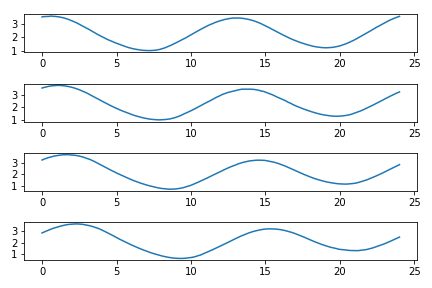
\includegraphics{images/fig2.png}
\caption{Figure\_2}
\end{figure}

    Use the \texttt{pd.find()} function to save the precipitation data
(number of inches only) exclusively for days in the year 2013 to a
vector NumPy array called \texttt{precip\_2013}. Use the plt.subplots()
method to plot the data in the first slot in Figure 1. Label its title,
and its y-axis as you see pictured in this document's Figure 1. Include
the grid lines as well. Allow b = '\&begin\_date=20180415'Python to
decide where your grid lines and axis tick marks should
be.\textbackslash{}

\begin{verbatim}
b = '&begin_date=20180415'
\end{verbatim}

You can aquire the data data for a different date by modifying the last
two numbers in the string
\texttt{b\ =\ \textquotesingle{}\&begin\_date=20180415\textquotesingle{}}.
For example, if we change the string to
\texttt{b\ =\ \textquotesingle{}\&begin\_date=20180416\textquotesingle{}},
we will acquire the data for April 16, 2018.

Find the title level data for four different days: April 15, April 16,
April 17 and April 18. Plot all four days as the same figure as four
subplots. You will need to change the \texttt{b} section of the url to
different values to pull down the data from different days.

For example, to get the data from year \texttt{2018}, month \texttt{04},
day \texttt{15} use:

\begin{verbatim}
b = '&begin_date=20180415'
\end{verbatim}

To get the data from year \texttt{2018}, month \texttt{04}, day
\texttt{16} use:

\begin{verbatim}
b = '&begin_date=20180416'
\end{verbatim}

The rest of the url is the same as the parts you used above to build the
first line plot.

    \begin{Verbatim}[commandchars=\\\{\}]
{\color{incolor}In [{\color{incolor}6}]:} \PY{n}{b} \PY{o}{=} \PY{l+s+s1}{\PYZsq{}}\PY{l+s+s1}{\PYZam{}begin\PYZus{}date=20180415}\PY{l+s+s1}{\PYZsq{}}
        \PY{n}{url} \PY{o}{=} \PY{n}{h} \PY{o}{+} \PY{n}{s} \PY{o}{+} \PY{n}{b} \PY{o}{+} \PY{n}{r} \PY{o}{+} \PY{n}{p} \PY{o}{+} \PY{n}{d} \PY{o}{+} \PY{n}{u} \PY{o}{+} \PY{n}{t} \PY{o}{+} \PY{n}{f}
        \PY{n}{url}
\end{Verbatim}


\begin{Verbatim}[commandchars=\\\{\}]
{\color{outcolor}Out[{\color{outcolor}6}]:} 'https://tidesandcurrents.noaa.gov/api/datagetter?station=9439040\&begin\_date=20180415\&range=24\&product=water\_level\&datum=STND\&units=metric\&time\_zone=lst\&format=csv'
\end{Verbatim}
            
    \begin{Verbatim}[commandchars=\\\{\}]
{\color{incolor}In [{\color{incolor}7}]:} \PY{k+kn}{import} \PY{n+nn}{pandas} \PY{k}{as} \PY{n+nn}{pd}
        \PY{n}{df15} \PY{o}{=} \PY{n}{pd}\PY{o}{.}\PY{n}{read\PYZus{}csv}\PY{p}{(}\PY{n}{url}\PY{p}{)}
        \PY{c+c1}{\PYZsh{}df16.head()}
        \PY{c+c1}{\PYZsh{}df16.columns}
\end{Verbatim}


    \begin{Verbatim}[commandchars=\\\{\}]
{\color{incolor}In [{\color{incolor}8}]:} \PY{n}{df15}\PY{o}{.}\PY{n}{drop}\PY{p}{(}\PY{p}{[}\PY{l+s+s1}{\PYZsq{}}\PY{l+s+s1}{ Sigma}\PY{l+s+s1}{\PYZsq{}}\PY{p}{,} \PY{l+s+s1}{\PYZsq{}}\PY{l+s+s1}{ O}\PY{l+s+s1}{\PYZsq{}}\PY{p}{,} \PY{l+s+s1}{\PYZsq{}}\PY{l+s+s1}{ F}\PY{l+s+s1}{\PYZsq{}}\PY{p}{,} \PY{l+s+s1}{\PYZsq{}}\PY{l+s+s1}{ R}\PY{l+s+s1}{\PYZsq{}}\PY{p}{,} \PY{l+s+s1}{\PYZsq{}}\PY{l+s+s1}{ L}\PY{l+s+s1}{\PYZsq{}}\PY{p}{,}\PY{l+s+s1}{\PYZsq{}}\PY{l+s+s1}{ Quality }\PY{l+s+s1}{\PYZsq{}}\PY{p}{]}\PY{p}{,} \PY{n}{axis}\PY{o}{=}\PY{l+m+mi}{1}\PY{p}{,} \PY{n}{inplace}\PY{o}{=}\PY{k+kc}{True}\PY{p}{)}
        \PY{n}{df15}\PY{o}{.}\PY{n}{columns} \PY{o}{=} \PY{p}{[}\PY{l+s+s1}{\PYZsq{}}\PY{l+s+s1}{date\PYZus{}time}\PY{l+s+s1}{\PYZsq{}}\PY{p}{,} \PY{l+s+s1}{\PYZsq{}}\PY{l+s+s1}{water\PYZus{}level}\PY{l+s+s1}{\PYZsq{}}\PY{p}{]}
        \PY{n}{df15}\PY{o}{.}\PY{n}{head}\PY{p}{(}\PY{p}{)}
\end{Verbatim}


\begin{Verbatim}[commandchars=\\\{\}]
{\color{outcolor}Out[{\color{outcolor}8}]:}           date\_time  water\_level
        0  2018-04-15 00:00        3.478
        1  2018-04-15 00:06        3.502
        2  2018-04-15 00:12        3.508
        3  2018-04-15 00:18        3.522
        4  2018-04-15 00:24        3.526
\end{Verbatim}
            
    \begin{Verbatim}[commandchars=\\\{\}]
{\color{incolor}In [{\color{incolor}9}]:} \PY{k+kn}{import} \PY{n+nn}{pandas} \PY{k}{as} \PY{n+nn}{pd}
        
        \PY{n}{b} \PY{o}{=} \PY{l+s+s1}{\PYZsq{}}\PY{l+s+s1}{\PYZam{}begin\PYZus{}date=20180418}\PY{l+s+s1}{\PYZsq{}}
        \PY{n}{url} \PY{o}{=} \PY{n}{h} \PY{o}{+} \PY{n}{s} \PY{o}{+} \PY{n}{b} \PY{o}{+} \PY{n}{r} \PY{o}{+} \PY{n}{p} \PY{o}{+} \PY{n}{d} \PY{o}{+} \PY{n}{u} \PY{o}{+} \PY{n}{t} \PY{o}{+} \PY{n}{f}
        \PY{n}{df} \PY{o}{=} \PY{n}{pd}\PY{o}{.}\PY{n}{read\PYZus{}csv}\PY{p}{(}\PY{n}{url}\PY{p}{)}
        \PY{n}{df}\PY{o}{.}\PY{n}{drop}\PY{p}{(}\PY{p}{[}\PY{l+s+s1}{\PYZsq{}}\PY{l+s+s1}{ Sigma}\PY{l+s+s1}{\PYZsq{}}\PY{p}{,} \PY{l+s+s1}{\PYZsq{}}\PY{l+s+s1}{ O}\PY{l+s+s1}{\PYZsq{}}\PY{p}{,} \PY{l+s+s1}{\PYZsq{}}\PY{l+s+s1}{ F}\PY{l+s+s1}{\PYZsq{}}\PY{p}{,} \PY{l+s+s1}{\PYZsq{}}\PY{l+s+s1}{ R}\PY{l+s+s1}{\PYZsq{}}\PY{p}{,} \PY{l+s+s1}{\PYZsq{}}\PY{l+s+s1}{ L}\PY{l+s+s1}{\PYZsq{}}\PY{p}{,}\PY{l+s+s1}{\PYZsq{}}\PY{l+s+s1}{ Quality }\PY{l+s+s1}{\PYZsq{}}\PY{p}{]}\PY{p}{,} \PY{n}{axis}\PY{o}{=}\PY{l+m+mi}{1}\PY{p}{,} \PY{n}{inplace}\PY{o}{=}\PY{k+kc}{True}\PY{p}{)}
        \PY{n}{df}\PY{o}{.}\PY{n}{columns} \PY{o}{=} \PY{p}{[}\PY{l+s+s1}{\PYZsq{}}\PY{l+s+s1}{date\PYZus{}time}\PY{l+s+s1}{\PYZsq{}}\PY{p}{,} \PY{l+s+s1}{\PYZsq{}}\PY{l+s+s1}{water\PYZus{}level}\PY{l+s+s1}{\PYZsq{}}\PY{p}{]}
        \PY{n}{df}\PY{o}{.}\PY{n}{head}\PY{p}{(}\PY{p}{)}
        \PY{n}{df18} \PY{o}{=} \PY{n}{df}\PY{o}{.}\PY{n}{copy}\PY{p}{(}\PY{p}{)}
\end{Verbatim}


    \begin{Verbatim}[commandchars=\\\{\}]
{\color{incolor}In [{\color{incolor}10}]:} \PY{k+kn}{import} \PY{n+nn}{matplotlib}\PY{n+nn}{.}\PY{n+nn}{pyplot} \PY{k}{as} \PY{n+nn}{plt}
         \PY{n}{fig}\PY{p}{,} \PY{p}{(}\PY{n}{ax1}\PY{p}{,}\PY{n}{ax2}\PY{p}{,}\PY{n}{ax3}\PY{p}{,}\PY{n}{ax4}\PY{p}{)} \PY{o}{=} \PY{n}{plt}\PY{o}{.}\PY{n}{subplots}\PY{p}{(}\PY{l+m+mi}{4}\PY{p}{,}\PY{l+m+mi}{1}\PY{p}{)}
         \PY{n}{ax1}\PY{o}{.}\PY{n}{plot}\PY{p}{(}\PY{n}{hours}\PY{p}{,}\PY{n}{df15}\PY{p}{[}\PY{l+s+s1}{\PYZsq{}}\PY{l+s+s1}{water\PYZus{}level}\PY{l+s+s1}{\PYZsq{}}\PY{p}{]}\PY{p}{)}
         \PY{n}{ax2}\PY{o}{.}\PY{n}{plot}\PY{p}{(}\PY{n}{hours}\PY{p}{,}\PY{n}{df16}\PY{p}{[}\PY{l+s+s1}{\PYZsq{}}\PY{l+s+s1}{water\PYZus{}level}\PY{l+s+s1}{\PYZsq{}}\PY{p}{]}\PY{p}{)}
         \PY{n}{ax3}\PY{o}{.}\PY{n}{plot}\PY{p}{(}\PY{n}{hours}\PY{p}{,}\PY{n}{df17}\PY{p}{[}\PY{l+s+s1}{\PYZsq{}}\PY{l+s+s1}{water\PYZus{}level}\PY{l+s+s1}{\PYZsq{}}\PY{p}{]}\PY{p}{)}
         \PY{n}{ax4}\PY{o}{.}\PY{n}{plot}\PY{p}{(}\PY{n}{hours}\PY{p}{,}\PY{n}{df18}\PY{p}{[}\PY{l+s+s1}{\PYZsq{}}\PY{l+s+s1}{water\PYZus{}level}\PY{l+s+s1}{\PYZsq{}}\PY{p}{]}\PY{p}{)}
         \PY{n}{plt}\PY{o}{.}\PY{n}{tight\PYZus{}layout}\PY{p}{(}\PY{p}{)}
         \PY{c+c1}{\PYZsh{}plt.savefig(\PYZsq{}images/fig2.png\PYZsq{}, dpi=72)}
         \PY{n}{plt}\PY{o}{.}\PY{n}{show}\PY{p}{(}\PY{p}{)}
\end{Verbatim}


    \begin{Verbatim}[commandchars=\\\{\}]

        ---------------------------------------------------------------------------

        NameError                                 Traceback (most recent call last)

        <ipython-input-10-280c93bc722b> in <module>
          2 fig, (ax1,ax2,ax3,ax4) = plt.subplots(4,1)
          3 ax1.plot(hours,df15['water\_level'])
    ----> 4 ax2.plot(hours,df16['water\_level'])
          5 ax3.plot(hours,df17['water\_level'])
          6 ax4.plot(hours,df18['water\_level'])
    

        NameError: name 'df16' is not defined

    \end{Verbatim}

    \begin{center}
    \adjustimage{max size={0.9\linewidth}{0.9\paperheight}}{combined_files/combined_18_1.png}
    \end{center}
    { \hspace*{\fill} \\}
    
    \hypertarget{y-y-plot}{%
\subsubsection{y-y plot}\label{y-y-plot}}

Use the \texttt{pd.find()} command to save some of the snow depth data
into a NumPy array called \texttt{winter13\_14\_sd}. Remember that the
column headers were in the Excel file. Refer to that file, if need be,
to see which column was for snow depth. Remember that we deleted the
date column and added 3 date columns in its place. Your data set should
only include the data from the first day of November 2013 to the last
day of February 2014. This will probably be the most difficult part of
this assignment.

Do the same to select the same days' snow fallen data and save it into a
NumPy array called \texttt{winter13\_14\_sf}. Use the
\texttt{ptl.plotyy()} command to plot both sets of data on the same
graph, but with different y-axes.

Notice the figure has a different vertical axis on the left from that on
its right. Let Matplotlib choose your axis limits and line colors. Be
sure to include the grid lines, x-axis label, y-axis label, title, and
legend you see pictured below.

\begin{figure}
\centering
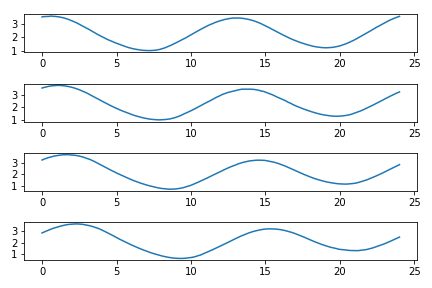
\includegraphics{images/fig2.png}
\caption{y-y plot}
\end{figure}

    \hypertarget{histogram}{%
\subsubsection{Histogram}\label{histogram}}

Create a Matplotlib Figure 3 that looks like this document's Figure 3.

Create a plot just like it from your \texttt{winter13\_14\_sf} NumPy
array. Match all of its labels etc. 20 bins were used to create this
histogram.

\begin{figure}
\centering
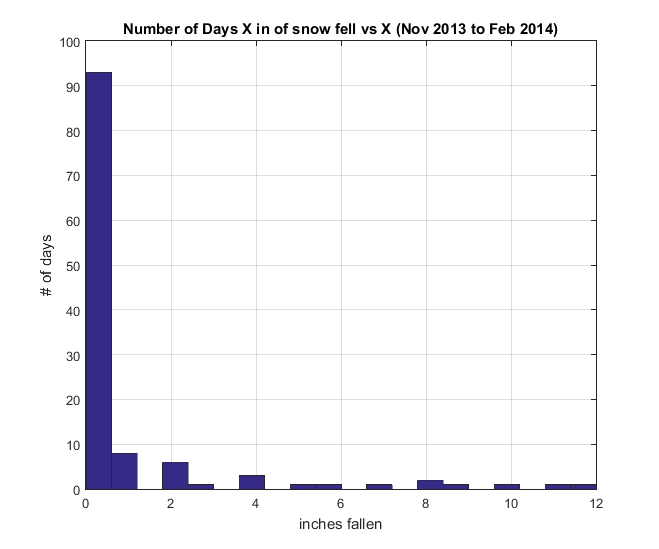
\includegraphics{images/fig3.png}
\caption{Histogram}
\end{figure}

    \hypertarget{deliverables}{%
\subsection{Deliverables}\label{deliverables}}

Each student's submission for the lab must be a single Jupyter Notebook.
The Jupyter Notebook must contain markdown cells that explain the code,
code cells that contain the code, and output cells that contain a total
of 3 plots. The three plots produced by the code cells in the notebook
should be:

\begin{itemize}
\item
  A plot that contains four sub-plots that shows level verses time
\item
  A y-y plot that shows snow level on one axis and rainfall on another
  axis
\item
  A histogram
\end{itemize}

Make sure to run all the cells in the Jupyter notebook before submitting
the file. Upload your \textbf{\emph{lab4.ipynb}} file to the Lab 4 drop
box in D2L.


    % Add a bibliography block to the postdoc
    
    
    
    \end{document}
